\documentclass{article}
\usepackage[a4paper, margin=2cm]{geometry}
\usepackage{xcolor}
\usepackage{xspace}
\usepackage{booktabs}
\usepackage{dsfont}
\usepackage{footmisc}
\usepackage{marvosym}
\usepackage{amsmath}
\usepackage{hyperref}
\usepackage[capitalise,noabbrev]{cleveref}
\usepackage{tabularx}
\usepackage{listings}
\usepackage{multirow}
\usepackage{pgfplots}
\usetikzlibrary{pgfplots.statistics}
\pgfplotsset{compat=newest}

\usepgfplotslibrary{groupplots}
\pgfplotsset{every axis/.style={scale only axis}}

\pgfplotsset{
  major grid style={thin,dotted},
  minor grid style={thin,dotted},
  ymajorgrids,
  yminorgrids,
  every axis/.append style={
    line width=0.7pt,
    tick style={
      line cap=round,
      thin,
      major tick length=4pt,
      minor tick length=2pt,
    },
  },
  legend cell align=left,
  legend style={
    line width=0.7pt,
    /tikz/every even column/.append style={column sep=3mm,black},
    /tikz/every odd column/.append style={black},
  },
  % move title closer
  legend style={font=\small},
  title style={yshift=-2pt},
  % less space on left and right
  enlarge x limits=0.04,
  every tick label/.append style={font=\footnotesize},
  every axis label/.append style={font=\small},
  every axis y label/.append style={yshift=-1ex},
  /pgf/number format/1000 sep={},
  axis lines*=left,
  xlabel near ticks,
  ylabel near ticks,
  axis lines*=left,
  label style={font=\footnotesize},
  tick label style={font=\footnotesize},
  plotMaximumLoadFactor/.style={
    width=36.0mm,
    height=35.0mm,
  },
}

\title{MPHF plot}
\date{}
\begin{document}
\definecolor{veryLightGrey}{HTML}{F2F2F2}
\definecolor{colorBmz}{HTML}{377EB8}
\definecolor{colorBdz}{HTML}{E41A1C}
\definecolor{colorFch}{HTML}{444444}
\definecolor{colorChd}{HTML}{000000}
\definecolor{colorChm}{HTML}{FF7F00}
\definecolor{colorHeterogeneous}{HTML}{4DAF4A}
\definecolor{colorPthash}{HTML}{984EA3}
\definecolor{colorRecSplit}{HTML}{A65628}
\definecolor{colorBbhash}{HTML}{F781BF}
\definecolor{lightGrey}{HTML}{DDDDDD}
\definecolor{colorSimdRecSplit}{HTML}{444444}
\definecolor{colorChd}{HTML}{377EB8}
\definecolor{colorRustFmph}{HTML}{A65628}
\definecolor{colorRustFmphGo}{HTML}{A65628}
\definecolor{colorRustPHast}{HTML}{FF5733}
\definecolor{colorSicHash}{HTML}{4DAF4A}
\definecolor{colorShockHash}{HTML}{F8BA01}

% IMPORT-DATA competitorNames _competitorNames.txt
% IMPORT-DATA queries comparison-N.txt

\centering
    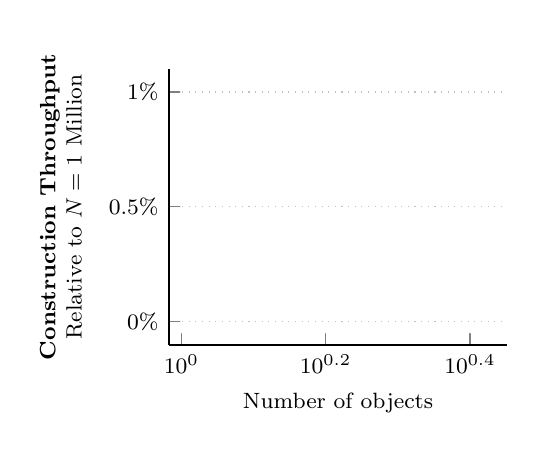
\begin{tikzpicture}
        \begin{axis}[
            plotMaximumLoadFactor,
            xlabel={Number of objects},
            ylabel={\begin{tabular}{c}\textbf{Construction Throughput}\\Relative to $N=1$ Million\end{tabular}},
            xmode=log,
            yticklabel={\pgfmathprintnumber\tick\%},
            width=43mm,
          ]
          %% MULTIPLOT(name, minimal|ptitle|attr)
          %% SELECT
          %%    N as x,
          %%    100.0*(N/AVG(constructionTimeMilliseconds))
          %%         / (SELECT MAX(avg) FROM (SELECT N/AVG(constructionTimeMilliseconds) AS avg FROM queries q WHERE queries.name = q.name AND queries.loadFactor=q.loadFactor GROUP BY N)) as y,
          %%    store_attr as attr,
          %%    store_name as ptitle,
          %%    IIF(minimal == 1, (name || 'Minimal'), name) AS detailed_name,
          %%    MULTIPLOT
          %% FROM queries
          %% JOIN competitorNames ON detailed_name = store_code
          %% GROUP BY name, minimal, N
          %% ORDER BY store_name,MULTIPLOT,x

          \legend{};
        \end{axis}
    \end{tikzpicture}
    \hspace{3mm}
    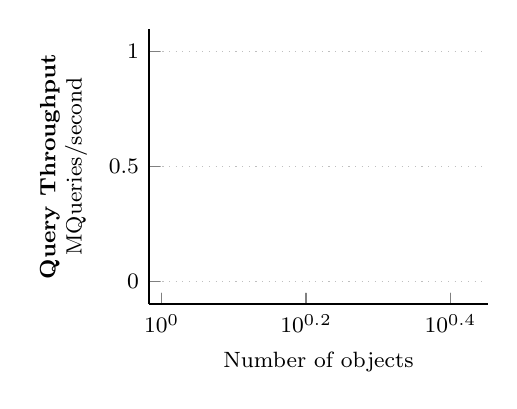
\begin{tikzpicture}
        \begin{axis}[
            plotMaximumLoadFactor,
            xlabel={Number of objects},
            ylabel={\begin{tabular}{c}\textbf{Query Throughput}\\MQueries/second\end{tabular}},
            legend columns=1,
            legend style={at={(1.1,0.5)},anchor=west},
            xmode=log,
            width=43mm,
          ]
          %% MULTIPLOT(name, minimal|ptitle|attr)
          %% SELECT
          %%    N as x,
          %%    .001*numQueries/AVG(queryTimeMilliseconds) as y,
          %%    store_attr as attr,
          %%    store_name as ptitle,
          %%    IIF(minimal == 1, (name || 'Minimal'), name) AS detailed_name,
          %%    MULTIPLOT
          %% FROM queries
          %% JOIN competitorNames ON detailed_name = store_code
          %% GROUP BY name, minimal, N
          %% ORDER BY store_name,MULTIPLOT,x

        \end{axis}
    \end{tikzpicture}

\end{document}

